\documentclass{llncs}

\providecommand{\event}{RuleML 2015} % Name of the event you are submitting to
\usepackage{aeguill}
\usepackage[utf8]{inputenc}
\usepackage[T1]{fontenc}
\usepackage{textcomp}
\usepackage{lmodern}
\usepackage[final]{microtype}
\usepackage{slashbox}
\usepackage{graphicx,xcolor}
\usepackage[draft]{changes}
%\usepackage[final]{changes}
\usepackage{listings}
\usepackage[linktocpage, colorlinks=true, linkcolor=blue, urlcolor=blue, citecolor=blue, %
             pdfkeywords={
                genomic annotation,
                network reconstruction,
                business rules,
                oriented object logic,
                four valued logic}]{hyperref}
\usepackage{filecontents}
\usepackage{float}
\usepackage{caption}
\usepackage{subcaption}
\usepackage{tikz}
\bibliographystyle{splncs03}
\pagestyle{headings}


\newcommand{\subsum}{\mathop{\raisebox{1ex}{$\cdot$}\!\!\!\!\leq}} 

\title{Reactive Graph Reasoning for Genomic Annotation}

\institute{Direction des Sciences du Vivant, CEA, Institut de Génomique, Genoscope, France \\
\and
CNRS-UMR8030, Evry, France \\
\and
Université d’Evry Val d’Essonne, Evry, France}

\author{Jonathan Mercier\inst{1}  \inst{3} \and David Vallenet\inst{1} \and Claudine Medigue\inst{1}  \inst{2}}

\begin{filecontents}{\jobname.bib}
    @article{mazumder2010community,
        title={Community annotation in biology},
        author={Mazumder, Raja and Natale, Darren A and Julio, Jessica Anne Ecalnir and Yeh, Lai-Su and Wu, Cathy H},
        journal={Biol Direct},
        volume={5},
        pages={12},
        year={2010}
    }
    @Article{vallenet2012microscope,
        author="Vallenet, D.  and Belda, E.  and Calteau, A.  and Cruveiller, S.  and Engelen, S.  and Lajus, A.  and Le Fevre, F.  and Longin, C.  and Mornico, D.  and Roche, D.  and Rouy, Z.  and Salvignol, G.  and Scarpelli, C.  and Thil Smith, A. A.  and Weiman, M.  and Medigue, C. ",
        title="{{M}icro{S}cope--an integrated microbial resource for the curation and comparative analysis of genomic and metabolic data}",
        journal="Nucleic Acids Res.",
        year="2013",
        volume="41",
        number="Database issue",
        pages="D636--647",
    }
    @incollection{belnap1977useful,
        title={A useful four-valued logic},
        author={Belnap Jr, Nuel D},
        booktitle={Modern uses of multiple-valued logic},
        pages={5--37},
        year={1977},
        publisher={Springer}
    }
    @misc{biolog,
        title={Biolog},
        author={Bochner, Barry R. and Barnby, Donald W.},
        journal={},
        howpublished="Website",
        url={http://www.biolog.com/products-static/phenotype\_microbial\_cells\_overview.php},
        year={}
    }
    @article{morgat2011unipathway,
        title={UniPathway: a resource for the exploration and annotation of metabolic pathways},
        author={Morgat, Anne and Coissac, Eric and Coudert, Elisabeth and Axelsen, Kristian B and Keller, Guillaume and Bairoch, Amos and Bridge, Alan and Bougueleret, Lydie and Xenarios, Ioannis and Viari, Alain},
        journal={Nucleic acids research},
        pages={gkr1023},
        year={2011},
        publisher={Oxford Univ Press}
    }
    @article{amir1999object,
        title={Object-oriented first-order logic},
        author={Amir, Eyal},
        journal={Linkiping Electronic Articles in Computer and Information Science (http://www.ida.liu.se/ext/etai)},
        url={http://www.ep.liu.se/ej/etai/1999/008/},
        pages={63--84},
        volume={4},
        year={1999}
    }
    @article{mcwhirter2001drools,
        title={Drools},
        author={McWhirter, Bob and others},
        howpublished="Website",
        pages={\href{http://drools.jboss.org}{drools.jboss.org}},
        year={2001}
    }
    @article{francke2005reconstructing,
        title={Reconstructing the metabolic network of a bacterium from its genome},
        author={Francke, Christof and Siezen, Roland J and Teusink, Bas},
        journal={Trends in microbiology},
        volume={13},
        number={11},
        pages={550--558},
        year={2005},
        publisher={Elsevier}
    }
    @article{proctor2008drools,
        title={Drools documentation},
        author={Proctor, Mark and Neale, Michael and Lin, Peter and Frandsen, Michael},
        journal={JBoss. org, Tech. Rep},
        year={2008}
    }
    @misc{phreak,
        title={PHREAK algorithm logic},
        author={Proctor, Mark},
        journal={},
        howpublished="Website",
        url={ https://www.google.fr/webhp?sourceid=chrome-instant\&ion=1\&espv=2\&ie=UTF-8#q=phreak+algorithm+logic},
        year={2013}
    }
    @article{sorokina2014profiling,
  title={Profiling the orphan enzymes},
  author={Sorokina, Maria and Stam, Mark and M{\'e}digue, Claudine and Lespinet, Olivier and Vallenet, David},
  journal={Biol. Direct},
  volume={9},
  number={10},
  year={2014}
}
@article{dagan2013genomes,
  title={Genomes of stigonematalean cyanobacteria (subsection V) and the evolution of oxygenic photosynthesis from prokaryotes to plastids},
  author={Dagan, Tal and Roettger, Mayo and Stucken, Karina and Landan, Giddy and Koch, Robin and Major, Peter and Gould, Sven B and Goremykin, Vadim V and Rippka, Rosmarie and de Marsac, Nicole Tandeau and others},
  journal={Genome biology and evolution},
  volume={5},
  number={1},
  pages={31--44},
  year={2013},
  publisher={Oxford University Press}
}
    
\end{filecontents}

\begin{document}
    
\definecolor{plantucolor0000}{RGB}{254,254,206}
\definecolor{plantucolor0001}{RGB}{168,0,54}
\definecolor{plantucolor0002}{RGB}{180,167,229}
\definecolor{plantucolor0003}{RGB}{0,0,0}
\definecolor{plantucolor0004}{RGB}{132,190,132}
\definecolor{plantucolor0005}{RGB}{3,128,72}
\definecolor{plantucolor0006}{RGB}{173,209,178}
\definecolor{plantucolor0007}{RGB}{200,41,48}
    
\maketitle

\begin{abstract}
Today's functional genomic knowledge is built from an incredible amount of genomes, whereas curation efforts to annotate them tend to decrease despite some community initiatives \cite{mazumder2010community}. To provide expert annotation as gold standard, bio-annotator community faced  big data issue need to be efficient.
To ease this manual process, we developed a Genomic Rule Oriented Object Logic System named GROOLS. It reconstruct metabolite networks from both automatic tasks and expert manual curating to provide a global view of predicted functions to bio-annotator. Thus, the community can to use the network context to annotate missing proteins. 
The combined use of a modern paradigm as an oriented object programming with the logic fields provide an interesting space of research. Complex biological information are pulled from various resources and represented as a structured object. These objects are bivalent, for a computer specialist, is an instance of a defined class, while for a logician is a theory.
Business rule coerce, control and make business decision. It separates clearly business logic from business application. A Business Rule Management System (BRMS) evaluates facts against a set of rules in a reproducible and efficient way.
This paper shows a standardized way to analyze and annotate genomes using a relevance logic and a hierarchical knowledge representation.
\keywords{genomic annotation, network reconstruction, business rules, oriented object logic, relevance logic, hierarchical knowledge representation}
\end{abstract}

\section{General description}
GROOLS is an applied research project mixing  biology, informatics and logic. It aim to standardize the use of biological results to annotate a genome. This expert system will highlight the bio-annotators on expected and unexpected gene annotation. Mining complex biological information to discovery new knowledge.\\
During analysis of a newly sequenced genome, the bio-annotator is facing the difficult task of checking the annotation consistency. Therefore, in such cases the bio-annotator should check the proteome against the biological knowledge about the organisms under study. However this is a colossal task and bio- annotator usually check sequence similarity to an already annotated protein to infer the gene annotation. The early stages are to understand the bio-annotator reasoning and the identification of a generic model. This generic model will be based on a predefined vocabulary.\\
A bio-annotator uses at least three types of fact. The first type is a ``prediction fact'', found with bioinformatics computing or bio-annotator analysis. The second one is an ``assertion fact'', an empirical evidence on organisms. The third is a trusted knowledge, a knowledge known to occur on one ore more organisms. A bio-annotator studying tryptophan autotroph organism will expect to found a tryptophan bio-synthesis pathway. The corresponding knowledge will therefore be marked accordingly as required. Reciprocally, if it is widely known to not grow on tryptophan free media which leads to the avoidance of the tryptophan bio-synthesis pathway. \\
Such reasoning system need a generic representation of the biological knowledge to be used on automatic genomic annotations. The BRMS used need to handle more than simple text message. Indeed, biological data are complex and structured with relations as ``is-a'' and ``has-a''. It needs to understand and reason such relation. \\
In order to obtain this kind of reasoning, we need to select resources, where facts come from. An asserted fact can come from biolog data \cite{biolog}, a trusted knowledge from unipathway \cite{morgat2011unipathway} and prediction from bioinformatics results or bio-annotator expertise from the Prokaryotic Genome DataBase (PkGDB) \cite{vallenet2012microscope}. \\
Trusted knowledge are gathered to form a graph. Prediction will influence the leafs of the graph while assertion influence the root of the graph. The prediction influences are spread from the leaf to the roots. Assertions and predictions facts can to take four different values. An assertion can take one of these word:  present, absent, both or unknown. While a prediction is assigned to one of these word: required, avoided, both or unknown. this set of word from a controlled vocabulary. These vocabularies are inferred to knowledges leading to a precise ending. This reconstruction of the metabolic network, aims to help bio-annotator to focus on missing gene annotations  \cite{francke2005reconstructing}.\\
This kind of logic is described by Belnap \cite{belnap1977useful} as a four valued logic. These theories are connected via some defined interface vocabularies. For each genome a set of rules is apply on a huge amount of biological knowledge to notify completeness and consistency. To achieve this we have applied the Object-Oriented First Order Logic (OOFOL) \cite{amir1999object} and extend it to a four valued logic. The four valued logic gives a finer analysis than the classic First Order Logic. Indeed, with the classic FOL, a non-observation is the same thing as non-existence.  This being so, from a biological point of view a false knowledge do not means the same thing than a not observed knowledge. In GROOLS, knowledge objects are theories which takes the form of a directed acyclic graph. Both ``assertion'' and ``prediction'' fact are an extension of a fact. They describe what is predicted or observed by experimentation.

\section{Genomic annotation}

Genomic annotation is one of most important task, once done we will be able to know organisms molecular physiology \replaced{and increase}{, increasing} our understanding of biological processes. This field aims to understand what an organism\deleted{s} is able to do \replaced{using a}{from} DNA sequence. The genome annotation unit process is the product of gene (protein). Understanding its function can lead to \replaced{novel}{new} discoveries. Some of these proteins are defined as enzymes, which means that they are able to catalyze at least one chemical reaction. The enzymatic product of these\deleted{s} chemical\deleted{s} reactions will be used by an enzyme, which by doing so gives some new products. This \replaced{chained-enzyme process}{enzyme chained process} is described by a metabolic pathway (Figure~\ref{fig:pathway}). To \replaced{create?}{form} a metabolic network, an enzyme can be depicted in more than one metabolic pathway.


\begin{figure}[H]
    \centering
    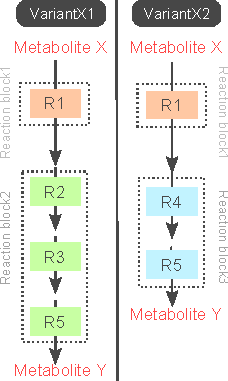
\includegraphics[width=0.5\textwidth]{img/metacycpathway.pdf}
    \caption{A metabolic pathway with two path to go from metabolite X to metabolite Y.}
    \label{fig:pathway}
\end{figure}

\replaced{In order to annotate several steps are done by a bio-annotator.}{A bio-annotator to annotate usually do several steps.} Commonly he defines a coding region, get\added{s} corresponding sequence, search\added{es} an homologous sequence and take\added{s} a look \replaced{at}{to} the genomic context to infer an annotation. In our opinion, \added{manual} genome annotation \deleted{task} is more \replaced{efficient once}{productive to be done after} an automatic genomic annotation \added{has been done}. Hence, it allows the reconstruction of \added{a (or change process into processes)} metabolic process (see \cite{francke2005reconstructing}), which is filled by automatic\deleted{s} tasks, and helps the bio-annotator to focus on missing genes. This automatic\deleted{s} gene annotation can be displayed with some other information\deleted{s},
enabling a better understanding of the organism abilities (depicted in Figure~\ref{fig:metabolicNetworkReconstruction}). By considering the following example, only the reaction\added{s} 1,3 and 5 are present, this leads to the conclusion that the Pathway X is not present. \replaced{manque la conclusion du if }{However if the studied organism is known to have the pathway X as described by some experimental information.} Bio-annotator point of view the pathway X is certainly present as a specific reaction occurring in the pathway X. Indeed\added{,} biological knowledge has some \added{je comprends pas le sens de hole }hole. Some enzymatic reaction\added{s} are known to occur into an organism\deleted{s} but these enzymes are bound to any genes, which is usually described as an orphan enzyme \cite{sorokina2014profiling}. This alternative reasoning is optimistic and fits better with our incomplete knowledge also known as pathway hole.

\begin{figure}[H]
    \centering
    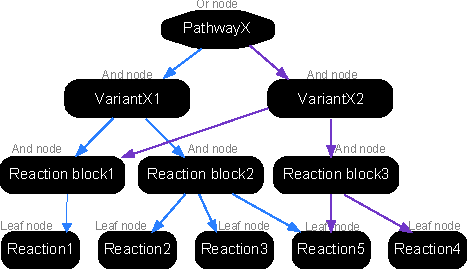
\includegraphics{img/pathway.pdf}
    \caption{Guided metabolic network reconstruction.}
    \label{fig:metabolicNetworkReconstruction}
\end{figure}

This kind of reasoning should \deleted{to} be done using up to twelve thousand genes \replaced{per}{by} organism\deleted{s} \cite{dagan2013genomes}. Moreover with the emergence of \replaced{next-generation sequencing}{next sequencing generation}, \replaced{DNA sequences are got faster than the annotation can be done.}{genome sequencing provides DNA sequence\added{s} in a shorter time frame quickly than bio-annotator community can do.} On the other hand\added{,} human expertise can lead to some inconsistencies which will be reused by other\deleted{s} bio-annotator\added{s}. To avoid \replaced{those}{these issues} we develop an expert system to automatize the bio-annotator reasoning. \added{In fact, }An automated reasoner can manage billions of facts in a standard and reproducible way.

\section{Benefits of applying an oriented-object expert system}
Biological facts are stored into many bio-data warehouse\deleted{, which are} typed to their corresponding characteristic\deleted{ to finally reason over}. For a computer scientist \replaced{this}{such} information \added{organisation} fits \added{with} an oriented object approach. An oriented object programming can \deleted{to} represent complex data by the use of classes and ease of handling \replaced{: each}{. Each} kind of data correspond\replaced{ing}{s} to a class. With the use of an object relational mapping, objects are automatically pulled \added{in}to a typed information from a data warehouse. An object is an instance of the corresponding class. A computer scientist will apply a formula, an algorithm, a reasoning, depending on the current \deleted{used} information type \added{used}. \\
We do not know in advance which type of object the end user will provide\deleted{s}. In order to communicate between these different type\added{s} of object\deleted{s}, the vocabulary is described by the use of interface. An interface provides a low coupling to have a well-structured computer system. Interfaces impose\deleted{s} communication protocols by defining a vocabulary. A class which implement\added{s} an interface\added{,} need\added{s} to implement\deleted{s} all vocabularies defined in the interface. \replaced{Also, an}{In other hand} interface avoid\added{s} multi-inheritance issues. To this end the set of rules use\added{s} the interface\deleted{s} to provide\deleted{s} a standardized vocabulary \replaced{for ?}{through} any type of object. Following the lowerCamelCase convention syntax (i.e getX, setX \dots), the use of inheritance interfaces define the commons accessors and mutators. Thus\added{,} attribute\replaced{d}{s} names are extractable in a standard way from various objects. We describe three generic\deleted{s} type\added{s} of fact\deleted{s}: Knowledge, Prediction and Assertion (Figure~\ref{fig:fact}) .

\begin{figure}[H]
    \centering
    \begin{subfigure}{0.6\textwidth}
    \includegraphics[width=\textwidth]{plantuml/fact.pdf}
    \caption{Generic Fact model.}
    \label{fig:fact}
    \end{subfigure}
    \hfill{}
    \begin{subfigure}{0.3\textwidth}
        \begin{lstlisting}[mathescape, basicstyle=\fontfamily{lmvtt}\selectfont]
FACT $\subsum$ TOP
id $\subsum$ toprole
name $\subsum$ toprole
nodeType $\subsum$ role
conclusion $\subsum$ role
evidence $\subsum$ role
KNOWLEDGE $\doteq$ ( and FACT
    ( atleast 0 partOf )
    ( some nodeType)
    ( some conclusion) )
OBSERVATION $\doteq$ ( and FACT
    ( some evidence ))
PREDICTION $\doteq$ ( and OBSERVATION )
ASSERTION $\doteq$ ( and OBSERVATION )
        \end{lstlisting}
    \caption{Logic formalism}
    \end{subfigure}
    \caption{Knowledge is used as a trusted information, a prediction is a bioinformatics result or a bio-annotator experiment, and an assertion as an empiric observation over our knowledge. Predictions and Assertions results are facing Knowledge.}
\end{figure}

JBoss DROOLS is an open rule-engine written in java \cite{proctor2008drools}. Natively an oriented-object language using a PHREAK algorithm \cite{phreak} to reason over a structured data. It does a \replaced{?}{nice} bridge between our java application and the logic paradigm.

\subsection{Reasoning over structured data}
\added{According to the} Logic point of view \added{,} a class is a structure \replaced{, an}{. An} instance of a class ( an object )\replaced{,}{ is} a theory. An object can \deleted{to} contain\deleted{s} other object\deleted{s}, that means a theory is a graph of smaller theories. Each theory \replaced{is}{are} defined by a coherent set of values. A class C is a tuple \( \langle \mathcal{L}_{C}, \mathcal{A}_{C} , \mathcal{I}_{C} \rangle \). Where  \(\mathcal{L} \) is the vocabulary (class methods) ,  \(\mathcal{A} \)  a set of axioms (attributes) and \(\mathcal{I} \) a set of vocabulary to implement (\( \mathcal{I}_{C} \subset\mathcal{L}_{C} \)). The truth of a sub-theory can be inferred to those upper theory following a Belnap logic. This logic is designed to cope with various and contradictory information sources. \replaced{In fact, }{Such that} if all \replaced{sub-theories}{sub-theory} are true then upper theories are true. if all \replaced{sub-theories}{sub-theory} are false then upper theories are false. If a set of \replaced{sub-theories}{sub-theory} are true and another false then \replaced{sub-theories}{sub-theory} take the value ``both''. \replaced{Finally, }{And also} if any information match a theory then the theory take the state ``neither'' (see Table~\ref{table:belnap}). In such case a ``and'' node have the following priority evaluation: false > both > none > true. As an example, a sub-theory S from a theory T representing a  ``and'' node. S is false then upper theory T is put to false. To the same line, priority evaluation for ``or'' node is: true > none > both > false.
    
\begin{table}[H]
    \caption{A four valued logic truth tables. T: true, F: false, B: both, N: none.\label{table:belnap}}
    \begin{minipage}{0.2\textwidth}
        \centering
        \begin{tabular}{|c||c|}\hline
            $F(\neg \alpha)$ & ~ \\ \hline \hline
            \textbf{T}       & F \\ \hline
            \textbf{B}       & B \\ \hline
            \textbf{N}       & N \\ \hline
            \textbf{F}       & T \\ \hline
        \end{tabular}
    \end{minipage}
    \begin{minipage}{0.35\textwidth}
        \centering
        \begin{tabular}{|c||c|c|c|c|c|c|}\hline
            $F(\land \alpha)$ & \textbf{T} & \textbf{B} & \textbf{N} & \textbf{F}  \\ \hline \hline
            \textbf{T}        & T          & B          & N          & F           \\ \hline
            \textbf{B}        & B          & B          & F          & F           \\ \hline
            \textbf{N}        & N          & F          & N          & F           \\ \hline
            \textbf{F}        & F          & F          & F          & F           \\ \hline
        \end{tabular}
    \end{minipage}
    \begin{minipage}{0.35\textwidth}
        \centering
        \begin{tabular}{|c||c|c|c|c|c|c|}\hline
            $F(\lor \alpha)$  & \textbf{T} & \textbf{B} & \textbf{N} & \textbf{F}  \\ \hline \hline
            \textbf{T}        & T          & T          & T          & T           \\ \hline
            \textbf{B}        & T          & B          & T          & B           \\ \hline
            \textbf{N}        & T          & T          & N          & N           \\ \hline
            \textbf{F}        & T          & B          & N          & F           \\ \hline
        \end{tabular}
    \end{minipage}
\end{table}


From the bio-annotator Point of view, there is some cases not as well covered by this logic. Indeed, if a required and not observed pathway X has at least one specific reaction (not shared to another reactions blocks)\replaced{, the}{. The} reaction block corresponding to this reaction can be considered as observed in the pathway X. Then the corresponding reaction block is set to present which infer the presence \replaced{of}{to} the pathway X. In this case\deleted{s}, we know the studied organism\deleted{s} has the required ability. Our knowledge is incomplete, with an optimistic Belnap's logic, a non observed pathway become observed. To do this, the ``and'' node priority evaluation has been modified  to true > false > both > none.

\subsection{Hierarchical knowledge representation}
A pathway can be represented  as a directed acyclic graph. In the following manner, a pathway contains one or more pathway variant\replaced{, a}{. A} pathway variant contains one or more reaction blocks\replaced{, }{. And}a reaction block contains one or more enzymatic reactions \replaced{and those}{, these} enzymatic reactions appear in one or more reaction blocks (as the reaction 3 in Figure~\ref{fig:metabolicNetworkReconstruction}). These knowledge\added{s} need to be studied, to know \deleted{if }their presence or absence in the given organism. Prediction fact\added{s} will infer in a bottom-up way while assertion fact\added{s} will do it in a top-down way. Once all facts are spread\deleted{s} over the DAG of knowledge a refined conclusion is put on each knowledge. This conclusion will be opposed to an assertion fact with a prediction fact comparing a four valued logic to an another \replaced{according to}{following} the conclusion table~\ref{table:conclusion}.


\begin{table}[H]
    \caption{Conclusion truth table.}
    \begin{tabular}{|l||*{4}{l|}}\hline
        \backslashbox{\textbf{Assertion}}{\textbf{Prediction}} & \makebox[6em]{\textbf{TRUE}} & \makebox[6em]{\textbf{FALSE}} & \makebox[6em]{\textbf{BOTH}} &\makebox[6em]{\textbf{UNKNOWN}} \\ \hline \hline
        \textbf{REQUIRED}                                      & Confirmed P.                 & Unexpected A.                 & Contradictory A.             & Missing                        \\ \hline
        \textbf{AVOIDED}                                       & Unexpected A.                & Confirmed A.                  & Contradictory P.             & Confirmed A.                   \\ \hline
        \textbf{BOTH}                                          & Ambiguous P.                 & Ambiguous A.                  & Ambiguous C.                 & Ambiguous.                     \\ \hline
        \textbf{UNKNOWN}                                       & Unconfirmed P.               & Unconfirmed A.                & Unconfirmed C.               & Unknown                        \\ \hline
    \end{tabular}
    
    \begin{tabular}{|l|l|}
        \multicolumn{2}{c}{Legend}  \\ \hline
        A. & Absence       \\ \hline
        P. & Presence      \\ \hline
        C. & Contradictory \\ \hline
    \end{tabular}
    \label{table:conclusion}
\end{table}


\section{Conclusion and future work}

Our genomic annotation reasoner provides an efficient and standardized way to reconstruct\deleted{ing} metabolic network. On each organism\deleted{s}, billions known proteins infer their functions to the corresponding gene. Bio-Annotator can focus their expertize on a smaller set of genes. Inconsistencies are detected and raised automatically to the bio-annotator to stop the spread of erroneous gene annotations. Using metabolic network reconstruction\added{,} data are \replaced{displayed}{visualizable} in a biological sense. Each knowledge (node of the network) has a refined conclusion.\\
To workaround knowledge hole we will focus our work on filling more accurate and relevant genome annotations.Thanks to months of support of the Grools systems meet complex demands of the bio-annotator community. 

\bibliography{\jobname}


\end{document}

